\documentclass[12pt,letterpaper]{article}
\usepackage{graphicx,textcomp}
\usepackage{natbib}
\usepackage{setspace}
\usepackage{fullpage}
\usepackage{color}
\usepackage[reqno]{amsmath}
\usepackage{amsthm}
\usepackage{fancyvrb}
\usepackage{amssymb,enumerate}
\usepackage[all]{xy}
\usepackage{endnotes}
\usepackage{lscape}
\newtheorem{com}{Comment}
\usepackage{float}
\usepackage{hyperref}
\newtheorem{lem} {Lemma}
\newtheorem{prop}{Proposition}
\newtheorem{thm}{Theorem}
\newtheorem{defn}{Definition}
\newtheorem{cor}{Corollary}
\newtheorem{obs}{Observation}
\usepackage[compact]{titlesec}
\usepackage{dcolumn}
\usepackage{tikz}
\usetikzlibrary{arrows}
\usepackage{multirow}
\usepackage{xcolor}
\newcolumntype{.}{D{.}{.}{-1}}
\newcolumntype{d}[1]{D{.}{.}{#1}}
\definecolor{light-gray}{gray}{0.65}
\usepackage{url}
\usepackage{listings}
\usepackage{color}
\usepackage{subcaption} %new, added by me

\definecolor{codegreen}{rgb}{0,0.6,0}
\definecolor{codegray}{rgb}{0.5,0.5,0.5}
\definecolor{codepurple}{rgb}{0.58,0,0.82}
\definecolor{backcolour}{rgb}{0.95,0.95,0.92}

\lstdefinestyle{mystyle}{
	backgroundcolor=\color{backcolour},   
	commentstyle=\color{codegreen},
	keywordstyle=\color{magenta},
	numberstyle=\tiny\color{codegray},
	stringstyle=\color{codepurple},
	basicstyle=\footnotesize,
	breakatwhitespace=false,         
	breaklines=true,                 
	captionpos=b,                    
	keepspaces=true,                 
	numbers=left,                    
	numbersep=5pt,                  
	showspaces=false,                
	showstringspaces=false,
	showtabs=false,                  
	tabsize=2
}
\lstset{style=mystyle}
\newcommand{\Sref}[1]{Section~\ref{#1}}
\newtheorem{hyp}{Hypothesis}

\title{Problem Set 1}
\date{Due: October 9, 2025}
\author{Applied Stats/Quant Methods 1}

\begin{document}
	\maketitle
	
	\section*{Instructions}
	\begin{itemize}
	\item Please show your work! You may lose points by simply writing in the answer. If the problem requires you to execute commands in \texttt{R}, please include the code you used to get your answers. Please also include the \texttt{.R} file that contains your code. If you are not sure if work needs to be shown for a particular problem, please ask.
\item Your homework should be submitted electronically on GitHub.
\item This problem set is due before 23:59 on Thursday October 9, 2025. No late assignments will be accepted.
	\end{itemize}
	
	\vspace{1cm}
	\section*{Question 1: Education}

A school counselor was curious about the average of IQ of the students in her school and took a random sample of 25 students' IQ scores. The following is the data set:\\
\vspace{.5cm}

\lstinputlisting[language=R, firstline=36, lastline=36]{PS01.R}  

\vspace{1cm}

\begin{enumerate}
	\item Find a 90\% confidence interval for the average student IQ in the school.\\
	
	\item Next, the school counselor was curious  whether  the average student IQ in her school is higher than the average IQ score (100) among all the schools in the country.\\ 
	
	\noindent Using the same sample, conduct the appropriate hypothesis test with $\alpha=0.05$.
\end{enumerate}

\newpage
\subsection*{Solution to Question 1}

\begin{enumerate}
	\item The 90\% confidence interval of the random sample of 25 students’ IQ scores lies between 94.99 and 101.89.\\
	
		\subitem{My code:}
		\lstinputlisting[language=R, firstline=38, lastline=48]{PS01.R}
	\item There is not enough statistical evidence to conclude that the average IQ of students at this school is higher than the national average of 100, as the calculated $t$-statistic (-0.596) is not greater than the critical t-value (1.711)\\
	
		\subitem{My code:}
		\lstinputlisting[language=R, firstline=53, lastline=62]{PS01.R}
\end{enumerate}
\newpage

\section*{Question 2: Political Economy}

\noindent Researchers are curious about what affects the amount of money communities spend on addressing homelessness. The following variables constitute our data set about social welfare expenditures in the USA. \\
\vspace{.5cm}


\begin{tabular}{r|l}
	\texttt{State} &\emph{50 states in US} \\
	\texttt{Y} & \emph{per capita expenditure on shelters/housing assistance in state}\\
	\texttt{X1} &\emph{per capita personal income in state} \\
	\texttt{X2} &  \emph{Number of residents per 100,000 that are "financially insecure" in state}\\
	\texttt{X3} &  \emph{Number of people per thousand residing in urban areas in state} \\
	\texttt{Region} &  \emph{1=Northeast, 2= North Central, 3= South, 4=West} \\
\end{tabular}

\vspace{.5cm}
\noindent Explore the \texttt{expenditure} data set and import data into \texttt{R}.
\vspace{.5cm}
\lstinputlisting[language=R, firstline=69, lastline=69]{PS01.R}  
\vspace{.5cm}
\begin{enumerate}

\item
Please plot the relationships among \emph{Y}, \emph{X1}, \emph{X2}, and \emph{X3}? What are the correlations among them (you just need to describe the graph and the relationships among them)?
\vspace{.5cm}
\item
Please plot the relationship between \emph{Y} and \emph{Region}? On average, which region has the highest per capita expenditure on housing assistance?
\vspace{.5cm}
\item
Please plot the relationship between \emph{Y} and \emph{X1}? Describe this graph and the relationship. Reproduce the above graph including one more variable \emph{Region} and display different regions with different types of symbols and colors.
\end{enumerate}
\newpage
\subsection*{Solution to Question 2}

\begin{enumerate}
	\item The scatterplot matrix reveals no strong or clear-cut correlations among the variables. However, a few moderate linear relationships are noteworthy:
		\begin{itemize}
			\item \emph{Y} and \emph{X1} show a moderately positive linear relationship, suggesting that states with higher per capita income tend to spend more on shelters and housing assistance.
			\item \emph{X1} and \emph{X3} also appear moderately positively correlated, indicating that higher-income states may have more urbanised populations.
			\item \emph{X2} does not exhibit any obvious linear relationship with the other variables, implying that financial insecurity may not be directly associated with expenditure, income, or urbanisation in a consistent way.
			\item \emph{X3} and \emph{Y} show a weak positive linear trend, suggesting that more urbanised states might spend slightly more on housing assistance, though the relationship is not strong.
		\end{itemize}
		\begin{figure}[h] 
			\centering
			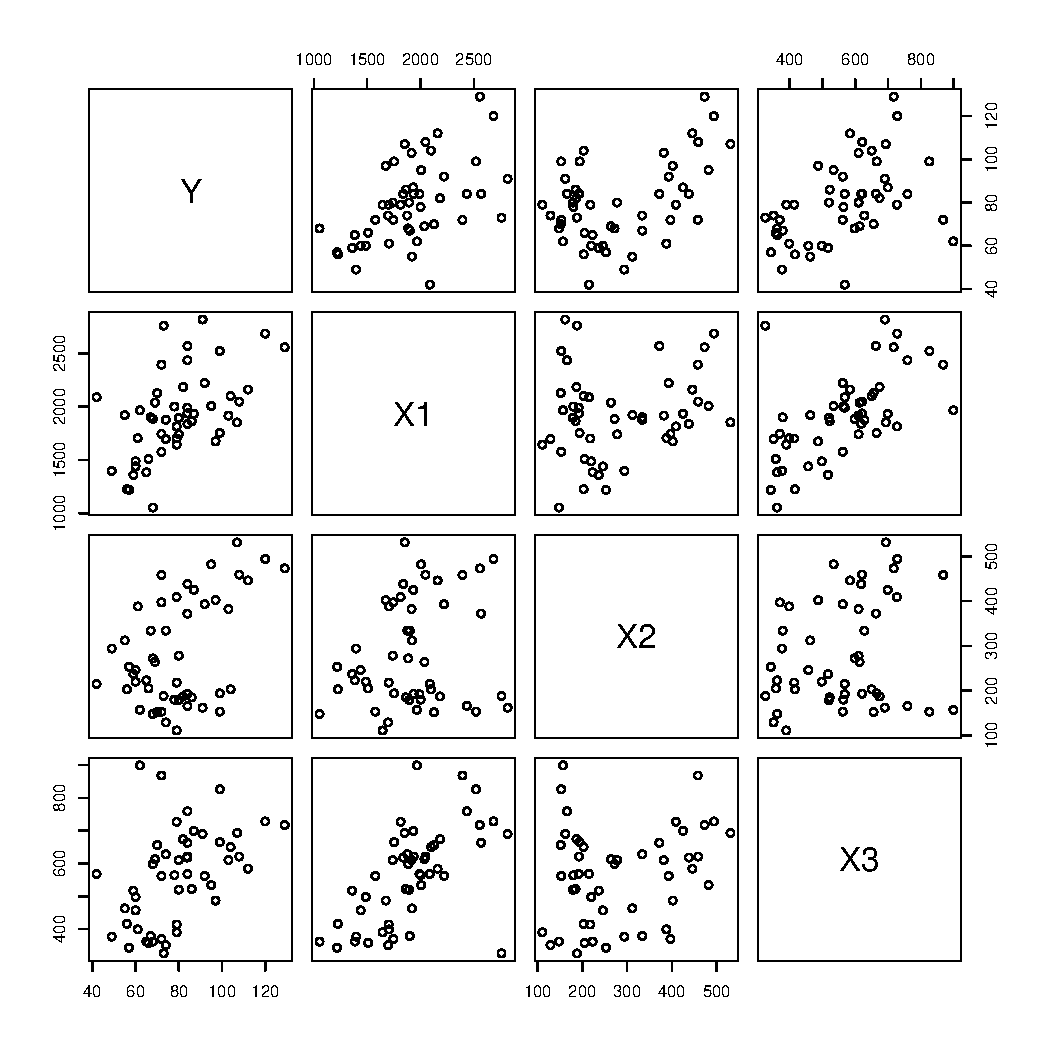
\includegraphics[width=0.45\linewidth]{pairs_plot_2_1.pdf}
			\caption{Scatterplot matrix of selected variables}
		\end{figure}
		\subitem{My code:}
		\lstinputlisting[language=R, firstline=68, lastline=75]{PS01.R} 
	\newpage
	\item On average, the region \textit{West} (4) has the highest expenditure on housing assistance.\\
		\begin{figure}[h] 
			\centering
			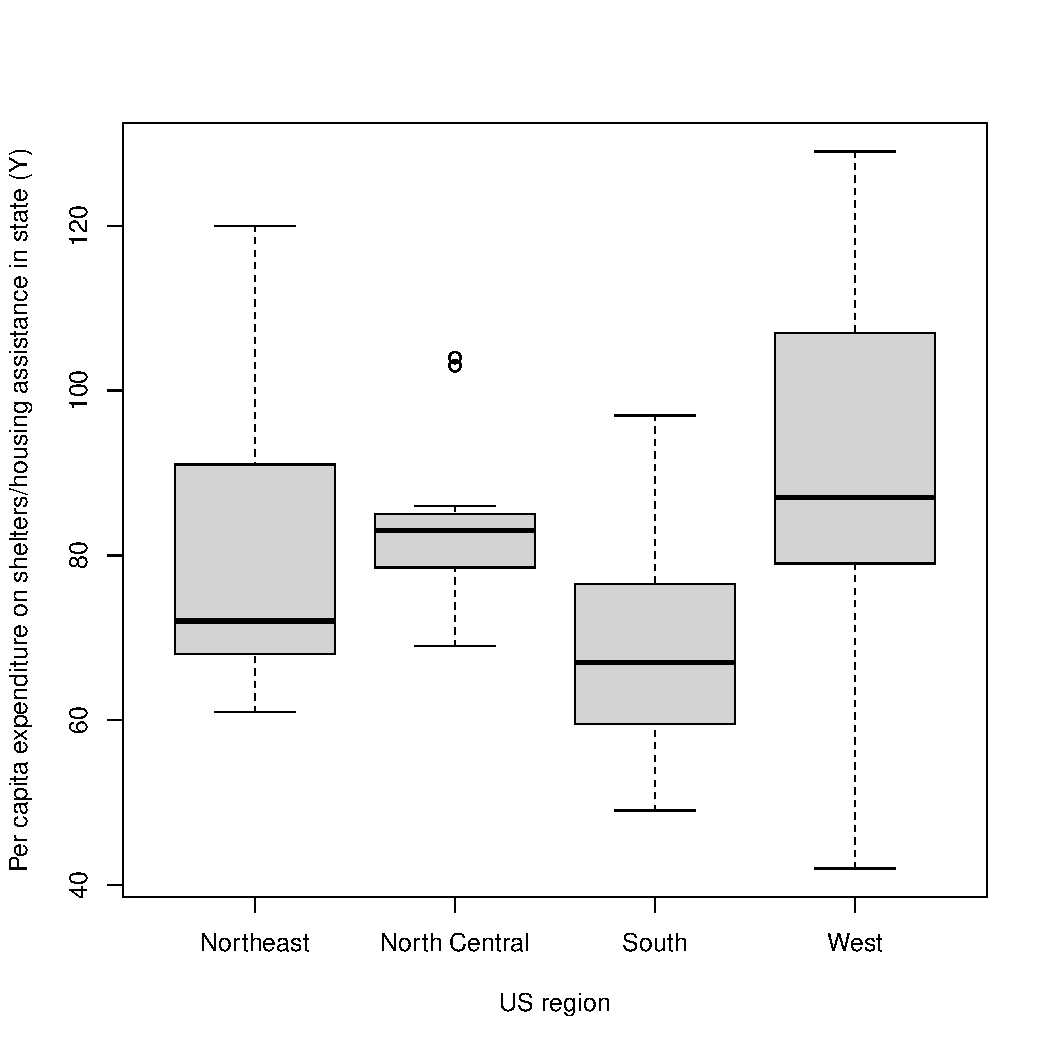
\includegraphics[width=0.6\linewidth]{box_plot_2_2.pdf}
			\caption{Boxplot showing \emph{Y} by \emph{Region}}
		\end{figure}
		\subitem{My code:}
		\lstinputlisting[language=R, firstline=83, lastline=88]{PS01.R} 
	\newpage
	\item \emph{Y} and \emph{X1} show a moderately positive linear relationship, suggesting that states with higher per capita income tend to spend more on shelters and housing assistance.\\
		\begin{figure}[h]
			\centering
			\begin{subfigure}{0.48\textwidth}
				\centering
				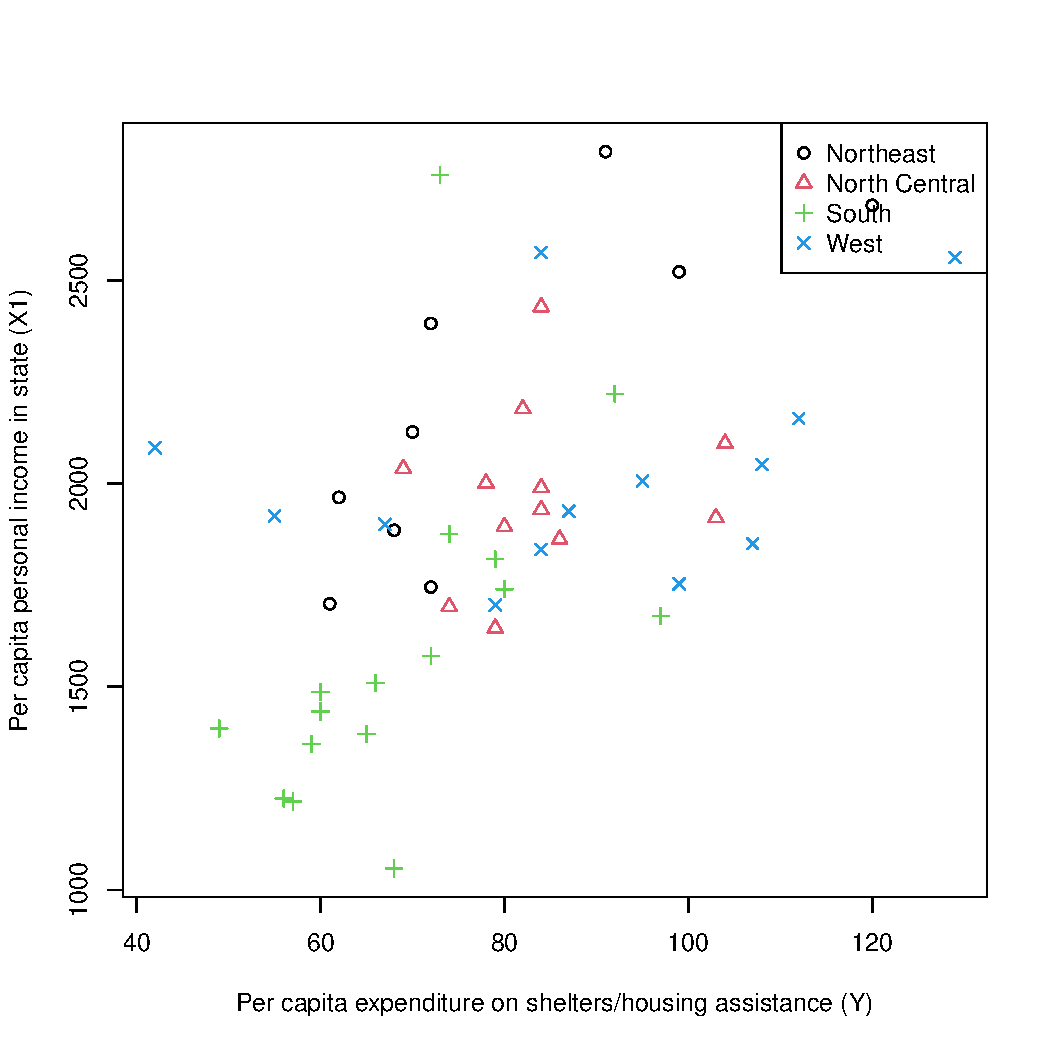
\includegraphics[width=\linewidth]{scatter_plot_2_3b.pdf}
				\caption{Scatterplot of \emph{X1} versus \emph{Y}, with points coloured and shaped by \emph{Region}.}
			\end{subfigure}
			\hfill
			\begin{subfigure}{0.48\textwidth}
				\centering
				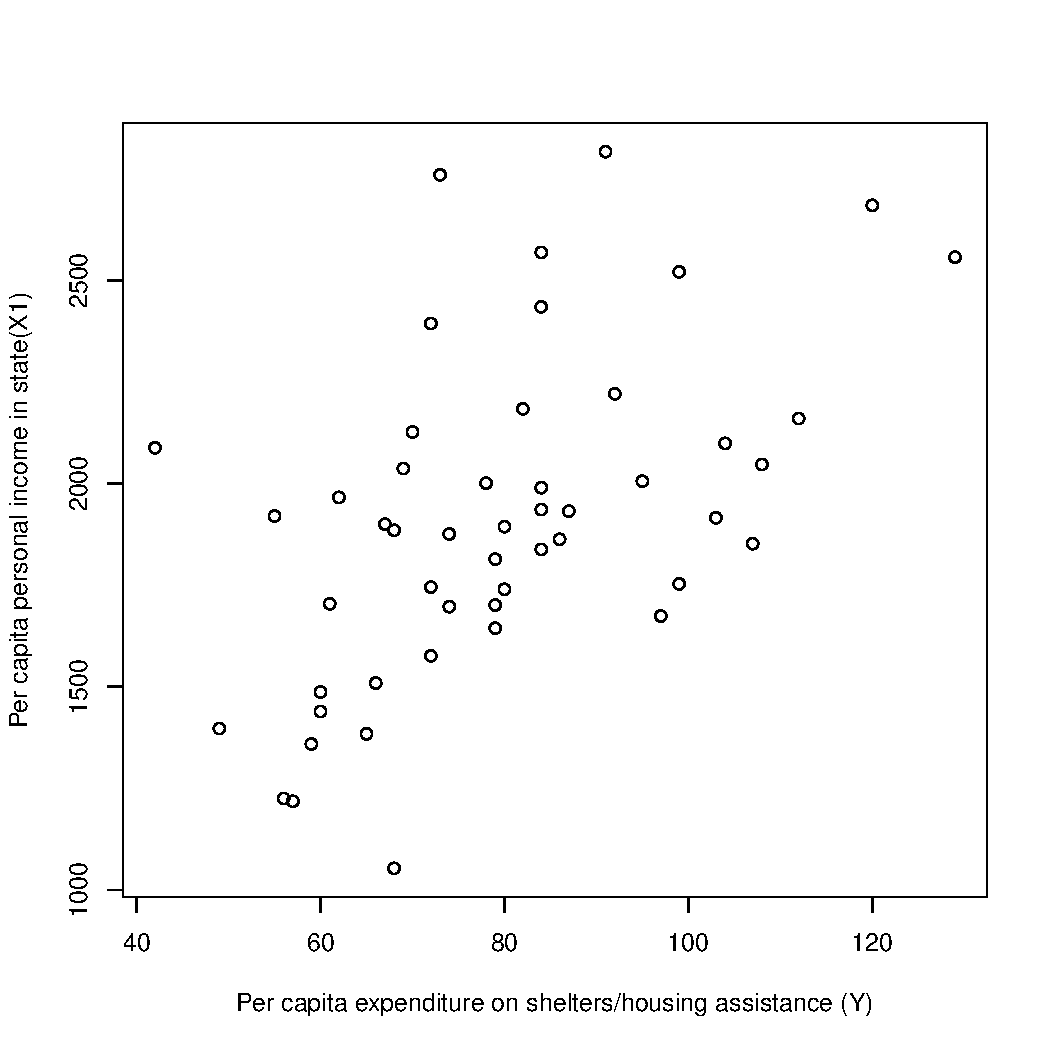
\includegraphics[width=\linewidth]{scatter_plot_2_3a.pdf}
				\caption{Scatterplot showing the relationship between \emph{X1} and \emph{Y}.}
			\end{subfigure}
		\end{figure}
		\subitem{My code:}
		\lstinputlisting[language=R, firstline=92, lastline=107]{PS01.R}
\end{enumerate}

\end{document}
